%!TEX TS-program = xelatex  
%!TEX encoding = UTF-8 Unicode
%%%%%%%%%%%%%%%%%%%%%%%%%%%%%%%%%%%%%%%%%%%%%%%%%%%%%%%%%%%%%%%%%%%%%%%%%%%%%
%                                                                           %
%   LaTeX File for Doctor (Master) Thesis of Shanghai Normal University     %
%   XeLaTeX              华东师范大学博士(硕士)论文模板                         %
%   Based on  Wang Tianshu's Template for XJTU (Version: 1.65)and           %
%         and Wu Yingnian's Template for Ncepubj University (LaTeXBook2.02).%
%                                                                           %
%   Last Update: 2014-10-10                                                 %
%   Tang Yincai, e-mail: yctang@stat.ecnu.edu.cn                            %
%%%%%%%%%%%%%%%%%%%%%%%%%%%%%%%%%%%%%%%%%%%%%%%%%%%%%%%%%%%%%%%%%%%%%%%%%%%%%

% 此模板在ctex2.9版本上测试通过, 请尽可能使用此版本
% 下载地址: http://www.ctex.org
% 此版本同样适合于Mac OS X系统的MacTeX, 这是此版更新的主要目的
% 下载地址: http://tug.org/mactex/

% 编译方式:    XeLaTeX 

\documentclass[12pt,openany,a4paper,twoside,UTF8]{ctexbook}
\usepackage{hyperref}
\hypersetup{%
%  dvipdfmx,% 设定要使用的 driver 为 dvipdfmx
  unicode={true},% 使用 unicode 来编码 PDF 字符串
  pdfstartview={FitH},% 文档初始视图为匹配宽度
  bookmarksnumbered={true},% 书签附上章节编号
  bookmarksopen={true},% 展开书签
  pdfborder={0 0 0},% 链接无框
  citecolor=blue,
  linkcolor=blue, % blue
  anchorcolor=green,
  urlcolor=blue,
  colorlinks=true,     %注释掉此项则交叉引用为彩色边框(将colorlinks和pdfborder同时注释掉)
  pdfborder=000        %注释掉此项则交叉引用为彩色边框
  %pdfstartview=FitH,
  %pdfpagemode=FullScreen % 实现打开后全屏
}
%============================ 引用的宏包 ==================================%
%!TEX TS-program = xelatex  
%!TEX encoding = UTF-8 Unicode

%%%%%%%%%%%%%%%%%%%%%%%%%%%%%%%%%%%%%%%%%%%%%%%%%%%%%%%%%%%%%%%%
%                   加载必要的宏包                             %
%%%%%%%%%%%%%%%%%%%%%%%%%%%%%%%%%%%%%%%%%%%%%%%%%%%%%%%%%%%%%%%%
\usepackage{xltxtra}
\setmainfont[BoldFont=黑体]{宋体}

\usepackage{amsmath,amsthm,amssymb,latexsym,xcolor}   % 使用AMS数学公式符号字体定理,页眉,扩展的color
\newcommand\hmmax{0} % default 3
\newcommand\bmmax{0} % default 4
\usepackage{bm}                                                % 希腊字母黑体显示
\usepackage{epsfig,graphicx,picinpar,subfigure,rotating}                  % 使用图形
\usepackage{fancybox,fancyvrb,shortvrb,fancyhdr}                                     % 支持抄录 --- 仅用于生成源代码
\usepackage{cite}  % natbib不能再用了:\usepackage[numbers,sort&compress]{natbib}
% %\usepackage{undertilde}
\usepackage{booktabs}      % 让你的表格中使用不同粗细的横线来划分行

\usepackage{flafter}            % 因为图形可浮动到当前页的顶部,所以它可能会出现
                                % 在它所在文本的前面. 要防止这种情况,可使用 flafter
                                % 宏包
\usepackage[below]{placeins}    %浮动图形控制宏包
                                %允许上一个section的浮动图形出现在下一个
                                %section的开始部分该宏包提供处理浮动对象
                                %的 \FloatBarrier 命令,使所有未处理的浮动
                                %图形立即被处理
\usepackage{array,tabularx,longtable,booktabs,threeparttable,colortbl,multirow,bigstrut}
\usepackage{dcolumn}            % 让表格中将小数点对齐
                                % 或 \hline\hline,当然在和垂直线的交叉处会有所不同。
%---%\usepackage{slashbox}           % 可在表格的单元格中画上一斜线。


%============================版面控制宏包=================================%
% 页边距:上:3.0cm,下:2.0cm,左:2.8cm,右:2.2cm,页眉:2.2cm,页脚1.5cm;
\usepackage[top=1.8cm,bottom=2cm,left=2.8cm,right=2.2cm,includehead,includefoot]{geometry}


%============================页眉页脚控制=================================%
\usepackage[symbol,perpage]{footmisc}  % 脚注控制可使得每页的脚注编码重新复位,
                                       % 但可能导致脚注的链接不正确
                                       % 注意大小写
% %\usepackage{pageno}                    % 章首页的页眉处理, 可以改为自己想要的形式

%======================== 数学公式相关宏包 ===============================%
\usepackage{mathtools}
\usepackage{mathrsfs}               % 不同于\mathcal or \mathfrak 之类的英文花体字体
\usepackage{subeqnarray}            %多个子方程(1-1a)(1-1b)
%\iffalse 以下是一个例子
%\begin{subeqnarray}
%\label{eqw} \slabel{eq0}
% x & = & a \times b \\
%\slabel{eq1}
% & = & z + t\\
%\slabel{eq2}
% & = & z + t
%\end{subeqnarray}
%\fi

%=============================标题与列表宏包=============================%
%\usepackage[sf]{titlesec}           % 控制标题的宏包,配合命令在后面,
                                    % 将cjk+miktex+scrbook+gb.cap下的章的标题号,
                                    % 比如~``第二章 XXX''位置于中心
\usepackage{enumerate}              % 改变列表标号样式宏包 其后可接选项[a,A,i,I,1]
\usepackage{caption2}               % 浮动图形和表格标题样式,可选项为
                                    % [scriptsize,footnotesize,centerlast]
\usepackage{setspace}               % 图形和表格的标题如果是多行,行距比较大,可以加宏包

%\usepackage{[small,compact]{titlesec}

%=========================== 特殊文本元素宏包 ==============================%
\usepackage{nicefrac}                % 在正文文本中排版分式时,可以用它来得到较好的排版效果。
\usepackage{units}                   % 基于 nicefrac 宏包,提供对计量单位比较美观的排版效果。
%\usepackage{titletoc}                % 控制目录的宏包
\usepackage{listings}                % 源代码宏包
\usepackage{makeidx}                 % 建立索引宏包
\makeindex

% ---------生成有书签的pdf及其开关
%\def\a{true}
%\ifx\a\useyap
%\AtBeginDvi{\special{pdf:tounicode GBK-EUC-UCS2}} % GBK -> Unicode
%\fi


%------公式,参考文献的标签显示在页边,在论文修改时可以使用------
%---%\usepackage{labname}               % 使用草稿专用宏包
%\usepackage[amsmath]{labelname}

\usepackage[subnum]{cases}           % 公式环境cases
%\usepackage{cases}


%\includeonly{body/intro}
\includeonly{preface/notation,body/intro,body/section,body/lists,body/table,body/graphs,body/equation,body/theorem,body/refes,body/conclud}

%\includeonly{body/intro,body/section,body/lists,body/table,body/graphs,body/equation,body/theorem,body/fonts,body/refes,body/conclud}

\pagestyle{fancy}
\setlength{\headheight}{20pt}
\hbadness=10000
\tolerance=10000

\begin{document}
\graphicspath{{figures/}}   %定义所有的eps文件在 figures 子目录下

%=========================== 文本格式定义 =================================%
%!TEX TS-program = xelatex  
%!TEX encoding = UTF-8 Unicode

%%%%%%%%%%%%%%%%%%%%%%%%%%%%%%%%%%%%%%%%%%%%%%%%%%%%%%%%%%%
%
% 主文档 格式定义
%
%%%%%%%%%%%%%%%%%%%%%%%%%%%%%%%%%%%%%%%%%%%%%%%%%%%%%%%%%%%


%自定义一个空命令, 用于注释掉文本中不需要的部分.
\newcommand{\comment}[1]{}

\allowdisplaybreaks
%\allowdisplaybreaks[n] %   n是1-4之间的数, 表示允许换页的程度,
                        %   比如\allowdisplaybreaks[0]表示可以换页但尽量不换,
                        %   而\allowdisplaybreaks[4]则是强制换页等同于\allowdisplaybreaks


%---------------------------- 数学公式设置 ------------------------------%
\setlength{\abovedisplayskip}{2pt plus1pt minus1pt}     %公式前的距离
\setlength{\belowdisplayskip}{2pt plus1pt minus1pt}     %公式后面的距离
\setlength{\arraycolsep}{2pt}   %在一个array中列之间的空白长度, 因为原来的太宽了


%===================================================================%
%                         各种标题样式
%===================================================================%
%======================= 标题名称中文化 ============================%
\renewcommand\contentsname{目\ 录}
\renewcommand\listfigurename{插\ 图\ 目\ 录}
\renewcommand\listtablename{表\ 格\ 目\ 录}
\renewcommand\bibname{参\ 考\ 文\ 献}    %book类型
\renewcommand\indexname{索\ 引}
\renewcommand\figurename{图}
\renewcommand\tablename{表}
%\renewcommand\partname{第\CJKnumber{\value{part}}部分}
%\renewcommand\chaptername{第\CJKnumber{\value{chapter}}章}

%=========================== 目录设置 ==================================%
\setcounter{tocdepth}{2}
\setcounter{secnumdepth}{2}

%---------------------- 定义章节的编号格式 --------------------------%
%\CTEXsetup[name={第,部分}]{part}
\CTEXsetup[name={第,章}]{chapter}
\CTEXsetup[number={\chinese{chapter}}]{chapter}
\CTEXsetup[name={\S,}]{section}
\CTEXsetup[name={\hspace{0em}\S,}]{subsection}
\CTEXsetup[name={\hspace{2\ccwd},}]{subsubsection}

%----------------------- 定义章节标题格式 ----------------------------%
%\titleformat{\appendix}[hang]{\normalfont\huge\filcenter\CJKfamily{hei}}
%    {\huge{\chaptertitlename}}{20pt}{\huge}
%\titlespacing{\appendix}{0pt}{-3ex  plus .1ex minus .2ex}{2.5ex plus .1ex minus .2ex}
%
%\titleformat{\chapter}[hang]{\normalfont\huge\filcenter\CJKfamily{hei}}
%    {\huge{\chaptertitlename}}{20pt}{\huge}
%\titlespacing{\chapter}{0pt}{-3ex  plus .1ex minus .2ex}{2.5ex plus .1ex minus .2ex}
%
%%\titleformat{\section}[hang]{\CJKfamily{hei}\Large \centering} %标题居中
%\titleformat{\section}[hang]{\CJKfamily{hei}\Large}
%    {\Large \thesection}{1em}{}{}
%\titlespacing{\section}
%    {0pt}{1.5ex plus .1ex minus .2ex}{\wordsep}
%
%\titleformat{\subsection}[hang]{\CJKfamily{hei}\large}
%    {\large \thesubsection}{1em}{}{}
%\titlespacing{\subsection}%
%    {0pt}{1.5ex plus .1ex minus .2ex}{\wordsep}
%
%\titleformat{\subsubsection}[hang]{\CJKfamily{hei}}
%    {\thesubsubsection }{1em}{}{}
%\titlespacing{\subsubsection}%
%    {0pt}{1.2ex plus .1ex minus .2ex}{\wordsep}



%====================== 定制图形和表格标题样式 =====================%
\renewcommand{\captionlabeldelim}{} %定义如  "图(表)2: 示例" 中的间隔符号,如 ":" ,这里定义为空
\renewcommand{\captionlabelsep}{\hspace{1em}} %定义图表编号与标题间的间隔距离
\renewcommand{\captionlabelfont}{\small \bf} %定义图表标签的字体
\renewcommand{\captionfont}{\small\rmfamily} %定义图表标题内容的字体

%--------------------- 定义图、表、公式的编号格式 -------------------%
%\numberwithin{equation}{section}  % used with amsmath package        %
%\numberwithin{table}{section}     % used with amsmath package        %
%\numberwithin{figure}{section}    % used with amsmath package        %
%------------------------ 定义图、表、公式的编号格式 ------------------------------%
\renewcommand{\thetable}{\arabic{chapter}-\arabic{table}}
\renewcommand{\theequation}{\arabic{chapter}-\arabic{equation}}
\renewcommand{\thefigure}{\arabic{chapter}-\arabic{figure}}

%%%@@@@@@@@@@@@@@@@@@@@@@@@@@@@@@@@@@@@@@@@@@@
%%%%%%%%%%%%%%%%%%%%%%%%%%%%%%%%%%%%%%%%%%%%%%%%%%%%%%%%
% 定义页眉和页脚 使用fancyhdr 宏包                     %
%%%%%%%%%%%%%%%%%%%%%%%%%%%%%%%%%%%%%%%%%%%%%%%%%%%%%%%%

\newcommand{\makeheadrule}{%
    \makebox[-3pt][l]{\rule[.7\baselineskip]{\headwidth}{0.4pt}}
    \rule[0.85\baselineskip]{\headwidth}{1.5pt}\vskip-.8\baselineskip}

\makeatletter
\renewcommand{\headrule}{%
    {\if@fancyplain\let\headrulewidth\plainheadrulewidth\fi
     \makeheadrule}}

%如果需要画单隔线, 则需要
\iffalse%-------------------------------%
\renewcommand{\headrulewidth}{0.5pt}    %在页眉下画一个0.5pt宽的分隔线
\renewcommand{\footrulewidth}{0pt}      % 在页脚不画分隔线.
\fi%------------------------------------%

\pagestyle{fancyplain}
\renewcommand{\chaptermark}[1]{%
\markboth{\CTEXthechapter\ #1}{}}
\renewcommand{\sectionmark}[1]{%
\markright{\S\thesection\ #1}}

\fancyhf{} %
\fancyfoot[C]{-\,\thepage\,-}
\fancyhead[LO]{\color{black}\CJKfamily{fs}\rightmark}
\fancyhead[RE]{\color{blue}\CJKfamily{fs}\leftmark}   % 在book文件类别下

%=============================== 脚注 =============================%
\renewcommand{\thefootnote}{\arabic{footnote}}



%====================================================================%
%          中文文档定理结构的设置,重定义一些正文相关标题             %
%                    针对中文稿设置                                  %
%====================================================================%

\newtheorem{definition}{\hspace{2\ccwd}{\bf{定义}}}[section]
\newtheorem{proposition}{\hspace{2\ccwd}{\bf{命题}}}[section]
\newtheorem{property}{\hspace{2\ccwd}{\bf{性质}}}[section]
\newtheorem{theorem}{\hspace{2\ccwd}{\bf{定理}}}[section]
\newtheorem{lemma}[theorem]{\hspace{2\ccwd}{\bf{引理}}}
\newtheorem{corollary}{\hspace{2\ccwd}{\bf{推论}}}  % 需要与定理一致的编号时用此命令
\newenvironment{cor}[1][\bf{推论}]{\newline\mbox{}\hspace{2\ccwd}\textbf{#1~~~}}{\hfill $\square$ \par}
\newtheorem{axiom}{\hspace{2\ccwd}{\bf{公理}}}[section]
%\newtheorem{exercise}{\hspace{2\ccwd}{\bf{习题}}}[chapter]
\newtheorem{exercise}{}[chapter]
\newtheorem{question}{\hspace{2\ccwd}{\bf{问题}}}
\newtheorem{example}{\hspace{2\ccwd}{\bf{例}}}[chapter]
%\newtheorem{exam}{\hspace{2\ccwd}例}[section]
\newtheorem{notation}{\hspace{2\ccwd}{\bf{记号}}}
\newtheorem{remark}{\hspace{2\ccwd}{\bf{注记}}}
\newtheorem{assumA}{{\bf 假设A-\hspace{-1mm}}}
\newtheorem{assumB}{{\bf 假设B-\hspace{-1mm}}}

\renewenvironment{proof}[1][证明]{\textbf{#1~~~}}{\hfill $\blacksquare$}
%\renewenvironment{proof}[1][Proof]{\textbf{#1.}}{\rule{0.5em}{0.5em}}
\newenvironment{solution}[1][解]{\textbf{#1~~~}}{\hfill $\blacksquare$} %{\hfill $\square$}
%\renewenvironment{proof}[1][Proof]{\textbf{#1.}}{\rule{0.5em}{0.5em}}


%=========================== 修改引用的格式 ==============================%

% 增加 \ucite 命令使显示的引用为上标形式
\newcommand{\ucite}[1]{\textsuperscript{\cite{#1}}}


%========================== 其它自定义 ==============================%

%====================================================================%
% 下面定义的命令(\alphtab \resettab)可以使表格编号变为 4-a, 4-b
% 使用说明:\alphtab 为开始产生处, \resettab为恢复原来表格编号形式处
% 这两个命令为自定义, 使用时应注意:不可放于 数学环境中!!!
% 在表格开始前和结束后使用!!!
%====================================================================%
%%\newcounter{savetab}%
%%\newcommand{\alphtab}{%
%%\setcounter{savetab}{\value{table}}%
%%\stepcounter{savetab}%
%%\setcounter{table}{0}%
%%%%\renewcommand{\thetable}{\arabic{savetab}-\alph{table}}%%article 中的定义
%%\renewcommand{\thetable}{\arabic{chapter}-\arabic{savetab}\alph{table}}}%%book 中的定义
%%%{\mbox{\arabic{table}-\alph{table}}}}%
%%
%%\newcommand{\resettab}{%
%%\setcounter{table}{\value{savetab}}%
%%%%\renewcommand{\thetable}{\arabic{table}}   %article 中的定义
%%\renewcommand{\thetable}{\arabic{chapter}-\arabic{table}}}  %book 中的定义


\def\defaultfont{\renewcommand{\baselinestretch}{1.5}
\fontsize{12pt}{13pt}\selectfont}



%%%%%%%%%%%%%%%%%%%%%%%%%%%%%%%%%%%%%%%%%%%%%%%%%%%%%%%%%%%%%%%%%%%%%%
% 封面、摘要、版权、致谢格式定义 --- by Feng Hua & Lei Wang
%%%%%%%%%%%%%%%%%%%%%%%%%%%%%%%%%%%%%%%%%%%%%%%%%%%%%%%%%%%%%%%%%%%%%%
\def\cdegree#1{\def\@cdegree{#1}}\def\@cdegree{}
%\def\ccovtitle#1{\def\@ccovtitle{#1}}\def\@ccovtitle{}
\def\ctitle#1{\def\@ctitle{#1}}\def\@ctitle{}
\def\caffil#1{\def\@caffil{#1}}\def\@caffil{}
\def\cmajor#1{\def\@cmajor{#1}}\def\@cmajor{}
\def\cstudy#1{\def\@cstudy{#1}}\def\@cstudy{}
\def\cauthor#1{\def\@cauthor{#1}}\def\@cauthor{}
\def\studentid#1{\def\@studentid{#1}}\def\@studentid{}
\def\csupervisor#1{\def\@csupervisor{#1}}\def\@csupervisor{}
%\def\cassosupervisor#1{\def\@cassosupervisor{~ & 副指导教师 & :& #1\\}}\def\@cassosupervisor{}
%\def\ccosupervisor#1{\def\@ccosupervisor{~ & 联\hfill 合\hfill 导\hfill 师 & :& #1\\}}\def\@ccosupervisor{}
\def\cdate#1{\def\@cdate{#1}}\def\@cdate{}
\long\def\cabstract#1{\long\def\@cabstract{#1}}\long\def\@cabstract{}
\def\ckeywords#1{\def\@ckeywords{#1}}\def\@ckeywords{}

%\def\ecovtitle#1{\def\@ecovtitle{#1}}\def\@ecovtitle{}
\def\edegree#1{\def\@edegree{#1}}\def\@edegree{}
\def\etitle#1{\def\@etitle{#1}}\def\@etitle{}
\def\eaffil#1{\def\@eaffil{#1}}\def\@eaffil{}
\def\emajor#1{\def\@emajor{#1}}\def\@emajor{}
\def\estudy#1{\def\@estudy{#1}}\def\@estudy{}
\def\eauthor#1{\def\@eauthor{#1}}\def\@eauthor{}
\def\esupervisor#1{\def\@esupervisor{#1}}\def\@esupervisor{}
\def\edate#1{\def\@edate{#1}}\def\@edate{}
\long\def\eabstract#1{\long\def\@eabstract{#1}}\long\def\@eabstract{}
\def\ekeywords#1{\def\@ekeywords{#1}}\def\@ekeywords{}

\def\makecover{
    \begin{titlepage}

% Chinese Cover

% 2013年度高校教师在职攻读硕士学位论文
    \parbox[t][4cm][c]{\textwidth}{\textbf{2013届研究生硕士学位论文}  \hfill 学校代码:~10269\hspace{3em}
    \\ \mbox{~~~~} \hspace{9.3cm}学\hphantom{校代}号:~YS00140203 }


    \parbox[t][5cm][t]{\textwidth}{
    \begin{center}

\includegraphics[height=2.2cm]{figures/ecnu_cn}
    \end{center} }

    \parbox[t][5cm][t]{\textwidth}{\Huge
    \begin{center} {\bf  \@ctitle } \end{center} }

    \parbox[t][6cm][c]{\textwidth}{ {\Large
    \begin{center}

    \renewcommand{\arraystretch}{1.0}
    \begin{tabular}{p{0cm}p{5em}l@{\extracolsep{1em}}l}
    ~ & 院\hfill 系 & & \underline{\@caffil } \\
    ~ & 专\hfill 业 & & \underline{\@cmajor}\\
    ~ & 研\hfill 究 \hfill 方 \hfill 向 & & \underline{\@cstudy}\\
    ~ & 导\hfill 师 & & \underline{\@csupervisor}\\
    ~ & 研\hfill 究 \hfill 生& & \underline{\@cauthor}\\
%    ~ & 学\hfill 号 & & \underline{\@studentid} \\
    ~ & 完\hfill 成\hfill 日\hfill 期 & & \underline{\@cdate}\\

    \end{tabular}
    \end{center} } }


    % 封二 空白页
    % English Cover
    \newpage

    \parbox[t][6cm][c]{\textwidth}{\textbf{Master Dissertation of Year 2013}  \hfill University ID:~10269\hspace{3em}
    \\ \mbox{~}\hspace{9.8cm}Student ID:~YS00140203 }

%    \parbox[t][2cm][t]{\textwidth}{
%    \begin{center}\end{center} }

    \parbox[t][4cm][t]{\textwidth}{\Huge
    \begin{center} {  \@etitle } \end{center} }

    \parbox[t][9cm][c]{\textwidth}{ {\large
    \begin{center}

    \renewcommand{\arraystretch}{1.3}
    \begin{tabular}{p{0cm}p{9em}l@{\extracolsep{1em}}l}
    ~ & Department & & \underline{\@eaffil } \\
    ~ & Major & & \underline{\@emajor}\\
    ~ & Research Direction & & \underline{\@estudy}\\
    ~ & Supervisor & & \underline{\@esupervisor}\\
    ~ & Author& & \underline{\@eauthor}\\
%    ~ & Number & & \underline{\@studentid} \\
    ~ & Date & & \underline{\@edate}\\
    \end{tabular} \end{center} } }

    \thispagestyle{empty}

    \end{titlepage}

    \normalsize

    %Authorization%%%%%%%%%%%%%%%%%%%%%%%%%%%%%%%%%%%%%%%%%%%%%%%%%%%
    \newpage

    \thispagestyle{empty}


\begin{minipage}[c]{0.95\textwidth}
{\LARGE \bf\centerline{华东师范大学学位论文原创性声明} }
\vskip0.3cm
{\normalsize\hspace{2\ccwd}郑重声明:本人呈交的学位论文《论文题目》, 是在华东师范大学攻读硕士/博士(请勾选)学位期间,
在导师的指导下进行的研究工作及取得的研究成果. 除文中已经注明引用的内容外, 本论文不包含其他个人已经发表或撰写过的研究成果.
对本文的研究做出重要贡献的个人和集体, 均已在文中作了明确说明并表示谢意. }
\end{minipage}
\parbox[t][1.5cm][c]{0.95\textwidth}{\large \hspace{3cm}
    作者签名: \hrulefill \hfill 日\hspace{2em}期: \hrulefill \hspace{1cm} }

\vskip0.7cm
\begin{minipage}[c]{0.95\textwidth}
{\LARGE \bf \centerline{华东师范大学学位论文著作权使用声明} }
\vskip0.3cm
{\normalsize\hspace{2\ccwd}《论文题目》系本人在华东师范大学攻读学位期间在导师指导下完成的硕士/博士
(请勾选)学位论文, 本论文的研究成果归华东师范大学所有. 本人同意华东师范大学根据相关规定保留和使用此学位论文,
并向主管部门和相关机构如国家图书馆、中信所和“知网”送交学位论文的印刷版和电子版;允许学位论文进入华东师范大学
图书馆及数据库被查阅、借阅;同意学校将学位论文加入全国博士、硕士学位论文共建单位数据库进行检索, 将学位论文的
标题和摘要汇编出版, 采用影印、缩印或者其它方式合理复制学位论文. }
\vskip0.3cm
\hspace{2\ccwd}本学位论文属于(请勾选)
\begin{enumerate}
\item[(\qquad)]1. 经华东师范大学相关部门审查核定的“内部”或“涉密”学位论文*,
 于\underline{\qquad}年\underline{\qquad}月\underline{\qquad}日解密, 解密后适用上述授权.
\item[(\qquad)]2. 不保密, 适用上述授权.
\end{enumerate}
\end{minipage}

\parbox[t][2.5cm][c]{0.95\textwidth}{\large \hspace{2cm}
作者签名:\hrulefill \hfill 导师签名:\hrulefill \hspace{1cm}
\\ \hspace*{2cm} 日\hspace{2em}期:\hrulefill \hfill 日\hspace{2em}期:\hrulefill \hspace{1cm} }
\vskip0.3cm\noindent
{\footnotesize * “涉密”学位论文应是已经华东师范大学学位评定委员会办公室或保密委员会审定过的学位论
文(需附获批的《华东师范大学研究生申请学位论文“涉密”审批表》方为有效),
未经上述部门审定的学位论文均为公开学位论文. 此声明栏不填写的, 默认为公开学位论文, 均适用上述授权). }

%Debating Group %%%%%%%%%%%%%%%%%%%%%%%%%%%%%%%%%%%%%%%%%%%%%%%%%%%

\newpage
\thispagestyle{empty}
\mbox{~~}
\vskip 3cm
\begin{center}
\textbf{\large XXX博士学位论文答辩委员会成员名单}
\end{center}
\begin{table}[h]
\begin{center}
\renewcommand{\arraystretch}{2.4}
  \begin{tabular}{|p{7em}|p{7em}|p{12em}|p{6em}|}
  \hline
  ~~~~姓~名  &  ~~~~职~称  &  \hspace{2em}单~~位  &  ~~~~备~注 \\ \hline
  & & & ~~~主~~席\\ \hline
  & & & \\ \hline
  & & & \\ \hline
  & & & \\ \hline
  & & & \\ \hline
  & & & \\ \hline
  & & & \\ \hline
  \end{tabular}
\end{center}
\end{table}


%Abstract and keywords%%%%%%%%%%%%%%%%%%%%%%%%%%%%%%%%%%%%%%%%%%%%%%%%%%%%%
\defaultfont

\setcounter{page}{0}
\normalsize
% !Mode:: "TeX:UTF-8"
% UTF-8 编辑器

%-------目录------------------------
\thispagestyle{empty} %取消当前页眉
%\setcounter{page}{1}

%目录中的点间距太大,改变 \@dotsep 的值可以减小
\makeatletter
    \renewcommand{\@dotsep}{0.8}
\makeatother

\newcommand{\loflabel}{图}
\newcommand{\lotlabel}{表}


\setcounter{tocdepth}{2}
\tableofcontents

% 插图目录
\renewcommand{\numberline}[1]{\loflabel~#1\hspace*{1em}}
\listoffigures

% 表格目录
\renewcommand{\numberline}[1]{\lotlabel~#1\hspace*{1em}}
\listoftables

%\listoffigures %显示所有插图目录
%\listoftables %显示所有表格目录
%显示所有定理类目录
%\listtheorems{definition}
%\listtheorems{example}
%\listtheorems{theorem}


    \chapter*{摘~~~~要}
    \addcontentsline{toc}{chapter}{\bf 摘~~~~要}
    \markboth{中~文~摘~要}{中~文~摘~要}

    \@cabstract

    \vspace{1em}

    \noindent {\bf 关键词:}\@ckeywords

    \defaultfont


    \chapter*{\textsf{\textbf{Abstract}}}
    \addcontentsline{toc}{chapter}{\bf ABSTRACT(英文摘要)}
    \markboth{英~文~摘~要}{英~文~摘~要}

    \@eabstract

    \vspace{1em}

    \noindent {\textbf{Key Words:}} \quad \@ekeywords
}


\long\def\acknowledge#1{
    \defaultfont

    \chapter*{致~~~~谢}
    \markboth{致谢}{致谢}
    \addcontentsline{toc}{chapter}{\bf 致谢}

    \begin{center}
    \parbox[t][8cm][t]{\textwidth}{{\hspace{2\ccwd}#1}}
    \end{center}
}



%============================== 封面 ======================================%
\renewcommand{\baselinestretch}{1.6}    %\baselineskip 的倍数,两者相乘为行间距。
\fontsize{14.75pt}{12pt}\selectfont     %\fontsize{size}{skip}skip相当于\baselineskip

%============================= 导言部分 ===================================%
\frontmatter        %导言部分页码自动为罗马数字
\sloppy             %放松拆行的限制解决中英文混排的断行问题,会加入间距,但
                    %不会影响断行
% !Mode:: "TeX:UTF-8"
% UTF-8 编辑器

\ctitle{{\bf 你的学位论文题目}}
\caffil{{\bf\makebox[4.5cm][s]{~金融与统计学院~}}}
\cmajor{{\bf\makebox[4.5cm][s]{概率论与数理统计}}}
\cstudy{{\bf\makebox[4.5cm][s]{~数~理~统~计~}}}
\csupervisor{{\bf\makebox[4.5cm][s]{某~某~某~~~~教~授}}}
\cauthor{{\bf\makebox[4.5cm][s]{~~李~~某~~}}}
\studentid{{\bf\makebox[4.5cm][s]{YS012345678}}}
\cdate{{\bf\makebox[4.5cm][s]{~2013年3月~}}}

%\edegree{Doctor of Science}
%\ecovtitle{{\textsf{EAST CHINA NORMAL UNIVERSITY}}\\ \\
%{\texttt{DISSERTATION TEMPLATE FOR DOCTOR/MASTER DEGREES}}}
\etitle{\bf\textsf{ TITLE OF YOUR DISSERTATION}}
\eaffil{{\bf \makebox[6.5cm][l]{Department of Statistics}}}
\emajor{\bf Probability and Mathematical Statistics}
\estudy{{\bf \makebox[6.5cm][l]{Mathematical Statistics}}}
\esupervisor{\bf \makebox[6.5cm][l]{Professor XXX}}
\eauthor{\bf \makebox[6.5cm][l]{LI XX}}
\edate{\bf \makebox[6.5cm][l]{March, 2013}}

\cabstract{
\renewcommand{\baselinestretch}{1.8}\normalsize
% !Mode:: "TeX:UTF-8"
% UTF-8 编辑器
% 中文摘要
此模板根据CTeX上提供的清泉(吴迎年, 华北电力大学)的博/硕士论文模板(LaTeXBook2.02)和
其它类似的论文模板(如清华大学博士/硕士论文模板)修改后完成. 2013之前的版本仅适用于Windows系统, 主要为BGK编码. 
2014版进行了进一步改进,以适用于不同的操作系统, 采用UTF-8编码, 且使用\XeLaTeX{}进行编译. 
目前它在Windows操作系统的CTeX2.9.x及Mac OSX的MacTeX测试通过. 

一般而言,中文摘要包含500-1000字,1-2页。关键词5-10个。

\ckeywords{论文,模板,博士,硕士,\LaTeX,CJK, XeLaTeX}
}


\eabstract{
\renewcommand{\baselinestretch}{1.8}\normalsize
% !Mode:: "TeX:UTF-8"
% UTF-8 编辑器

% 英文摘要
This template is based on Qinquan's Doctor/Master thesis template (LaTeXBook2.02)
and similar thesis templates (e.g. Tsinghua's Doctor/Master thesis template).
It has been tested under the full version of CTeX2.4.2 (with miktex2.4) or later.


Generally, the abstract and the key words should be consistent
with the Chinese version.

\ekeywords{thesis, template, doctor, master, \LaTeX, CJK}

}


       %封面 (含使用授权, 中文摘要, 英文摘要)

\makecover

%%目录
%\renewcommand{\baselinestretch}{1.5}
%\fontsize{12pt}{12pt}\selectfont


%符号对照表
% !Mode:: "TeX:UTF-8"
% UTF-8 编辑器

\defaultfont

\chapter*{主要符号对照表}
\addcontentsline{toc}{chapter}{\bf 主要符号对照表}
\markboth{主要符号对照表}{主要符号对照表}

\begin{tabular}{l@{\extracolsep{2em}}l}
Ph.D. & 哲学博士(Doctor of Philosophy)\\
M.S. & 理学硕士(Master of Science)
\end{tabular}


%=============================== 正文部分 ================================%
\mainmatter %进入正文页码自动变为阿拉伯数字章节计数器启动
% 对应于小四的标准字号是 12pt

%设置是正文各章使用的标准字体与行距
\renewcommand{\baselinestretch}{1.2}
\fontsize{11pt}{12pt}\selectfont

%正文章节 input不重新起一页,include重起一页
\setcounter{page}{1}

\include{body/intro}
% !Mode:: "TeX:UTF-8"
% UTF-8 编辑器
\chapter{章节层次}
\section{章节层次示例 }
\label{chap1:sample}
\setcounter{subsubsection}{0}
\section{章节层次示例 \label{chap2:sample}}
\section{章节层次示例 \label{chap3:sample}}
\subsection{章节层次示例 \label{chap3:chap1:sample}}
\subsection{章节层次示例 \label{chap3:chap2:sample}}
\subsection{章节层次示例 \label{chap3:chap3:sample}}
\subsection{章节层次示例 \label{chap3:chap4:sample}}
\subsubsection{章节层次示例 \label{chap3:chap4:chap1:sample}}
\subsubsection{章节层次示例 \label{chap3:chap4:chap2:sample}}
\subsubsection{章节层次示例 \label{chap3:chap4:chap3:sample}}
\subsubsection{章节层次示例 \label{chap3:chap4:chap4:sample}}

参见标题\ref{chap3:chap2:sample}

参见标题\ref{chap3:chap3:sample}

参见标题\ref{chap3:chap4:chap1:sample}

% !Mode:: "TeX:UTF-8"
% UTF-8 编辑器

%============================ 自定义文字块 ================================%
\newcommand{\aaa}{这是科技文稿排版测试这是科技文稿排版测试}

\chapter{列表 \label{chap4:liebiao}}
\section{有序列表 \label{chap4:chap1:bianhao}}
\subsection{嵌套的有序列表}
\begin{enumerate}
    \item {项目列表}
    \item {项目列表}
    \item {项目列表}
    \begin{enumerate}
        \item {项目列表}
        \item {项目列表}
        \item {项目列表}
        \begin{enumerate}
            \item {项目列表}
            \item {项目列表}
            \item {项目列表}
            \begin{enumerate}
            \item {项目列表}
            \item {项目列表}
            \item {项目列表}
            \end{enumerate}
        \end{enumerate}
    \end{enumerate}
\end{enumerate}

\subsection{带标号式样的有序列表}
% 使用enumerate宏包
\begin{enumerate}[{A}-i]
    \item \aaa
    \item \aaa
    \item \aaa
\end{enumerate}

\begin{enumerate}[{\bf 第}1{\bf 条}]
    \item \aaa
    \item \aaa
    \item \aaa
\end{enumerate}

\begin{enumerate}[a]
    \item \aaa
    \item \aaa
    \item \aaa
\end{enumerate}

\begin{enumerate}[I]
    \item \aaa
    \item \aaa
    \item \aaa
\end{enumerate}

\section{无序列表 \label{chap4:chap3:wubianhao}}

\begin{itemize}
\item {项目列表}
\item {项目列表}
    \begin{itemize}
    \item {项目列表}
    \item {项目列表}
    \item {项目列表}
        \begin{itemize}
        \item {项目列表}
        \item {项目列表}
        \item {项目列表}
        \end{itemize}
    \end{itemize}
\end{itemize}

\section{描述列表 \label{chap4:chap4:description}}

\begin{description}
    \item[描述列表] \aaa
    \item[描述列表] 描述列表
 \end{description}




% !Mode:: "TeX:UTF-8"
% UTF-8 编辑器
\chapter{表格样本}
\section{各种表格实例}
\subsection{无线表格,小数点对齐}
\tabbingsep=0pt
\begin{tabbing}
\heiti 行星\hspace{10mm}\=\heiti 赤道半径 km\hspace{10mm}
  \=\heiti 公转周期 d\\
\pushtabs
水星\hspace{20mm} \=  2\'.439\hspace{18mm}
\= 87\'.9\\
金星 \>      6\'.1  \> 224\'.682\\
地球 \> 6378\'.14 \> 365\'.25
\poptabs
\end{tabbing}
\subsection{固定列宽和自动伸缩列宽的三线表}
% 使用宏包booktabs---三线表
%%%%% ===== 固定列宽和自动伸缩列宽表格 ===========================================
% 修改\\, 否则必须用\tabularnewline代替\\
\newcommand{\PreserveBackslash}[1]{\let\temp=\\#1\let\\=\temp}
\newcolumntype{C}[1]{>{\PreserveBackslash\centering}p{#1}}
\newcolumntype{R}[1]{>{\PreserveBackslash\raggedleft}p{#1}}
\newcolumntype{L}[1]{>{\PreserveBackslash\raggedright}p{#1}}
\begin{table}[htbp]
  \centering\caption{\label{table:tab9}2000
           和~2004 年中国制造业产品的出口份额}
  \begin{tabular}{l*{2}{R{2cm}}}
  \toprule
    & 2000 & 2004 \\
  \midrule
    钢铁                  &  3.1 &  5.2 \\
    化学制品              &  2.1 &  2.7 \\
    办公设备及电信设备    &  4.5 & 15.2 \\
    汽车产品              &  0.3 &  0.7 \\
    纺织品                & 10.4 & 17.2 \\
    服装                  & 18.3 & 24.0 \\
  \bottomrule
  \end{tabular}
\end{table}


\subsection{跨页长表格: 使用 \texttt{longtable}宏包}
 \renewcommand{\arraystretch}{0.8}
\begin{longtable}{p{3cm}|p{8cm}}
\caption{统计分析中常用的函数与作用\label{ltab-1}}\\
 \toprule
 \rowcolor[gray]{.9}
统计函数 & 作用\\
 \midrule
$\max(x)$ &  返回向量x中最大的元素\\
$\min(x)$ & 返回向量x中最小的元素\\
$\texttt{which.max}(x)$ & 返回向量x中最大元素的下标\\
$\texttt{which.min}(x)$ & 返回向量x中最小元素的下标\\
$\texttt{mean}(x)$ & 计算样本(向量)x的均值\\
$\texttt{median}(x)$ & 计算样本(向量)x的中位数\\
$\texttt{mad}(x)$ & 计算中位绝对离差\\
$\texttt{var}(x)$ &  计算样本(向量)x的方差\\
$\texttt{sd}(x)$ & 计算向量x的标准差\\
$\texttt{range}(x)$ & 返回长度为2的向量: $\texttt{c}(\min(x),\max(x))$\\
$\texttt{IQR}(x)$ & 计算样本的四分位数极差\\
$\texttt{quantile}(x)$ & 计算样本常用的分位数\\
$\texttt{summary}(x)$ & 计算常用的描述性统计量(最小、最大、平均值、中位数和四分位数)\\
$\cdots$ & $\cdots$\\
  \bottomrule
\end{longtable}


\subsection{单元格合并}
\renewcommand{\multirowsetup}{\centering}
\begin{table}[htbp]
\centering
\caption{单元格合并}\label{merge}
\begin{tabular}{c|r|r}\hline
\multirow{3}[2]{20mm}{行星} & \multicolumn{2}{p{40mm}}%
{\centering 与太阳的距离 \\ (million km)}
\bigstrut[t] \\ \cline{2-3}
& \multicolumn{1}{c}{最远点}
& \multicolumn{1}{c}{最近点}
\bigstrut[t] \\ \hline
天王星 & 3011.0 & 2740.0 \bigstrut[t] \\
金星   & 109.0  & 107.6 \\
地球   & 152.6  & 147.4 \\ \hline
\end{tabular}
\end{table}


\subsection{带注释的表格: 使用threeparttable}

\begin{table}[h]
  \caption{2006-2007$^a$\tnote{}赛季科比布莱恩特投篮命中率的后验特征量
  \label{table:tab8}}
  \centering\small
\begin{threeparttable}[b]
\begin{tabular}{lccc}
\toprule
后验 & & 参数 &\\
\cline{2-4}
特征量 & 对数成败优势比$(\theta)$ & 成败优势比$(o)$ & 成功概率$(\pi)$\\
\midrule
均值 & -0.112 & 0.896 & 0.472\\
中位数 & -0.109 & 0.897 & 0.473\\
标准差 & 0.072 & 0.065 & 0.018\\
$Q_{2.5}$\tnote{b} & -0.261 & 0.770 & 0.435\\
$Q_{97.5}$ & 0.026 & 1.026 & 0.507\\
\bottomrule
\end{tabular}
{\tiny 说明:
\begin{tablenotes}
\item[a] 随机游动算法, 剔除期B=500次迭代; 被保留迭代次数$T'=2000$.
\item[b] $Q_{p}$表示分布的$p$分位数.
\end{tablenotes}}
\end{threeparttable}
\end{table}


%\section{表格自动编号}
%%\iffalse%%%%%%%%%%%%%%%%%%%%%%%%%%%%%%%%%%%%%%%%%%%%%%%%%%%
%
%\alphtab %产生形如 4-a,4-b 的编号
%\begin{table}[htbp]
%\begin{minipage}[htbp]{0.3\linewidth}
%  \centering
%  \caption{表格}\label{chap6:biaoge2}
%  \begin{tabular}{|c|c|c|}
%    \hline
%    % after \\: \hline or \cline{col1-col2} \cline{col3-col4} ...
%    123 & 4 & 5 \\
%    \hline
%    67 & 890 & 13 \\
%    \hline
%  \end{tabular}
%\end{minipage}
%\begin{minipage}[htbp]{0.3\linewidth}
%  \centering
%  \caption{表格}\label{chap6:biaoge3}
%  \begin{tabular}{|c|c|c|}
%    \hline
%    % after \\: \hline or \cline{col1-col2} \cline{col3-col4} ...
%    123 & 4 & 5 \\
%    \hline
%    67 & 890 & 13 \\
%    \hline
%  \end{tabular}
%\end{minipage}
%\begin{minipage}[htbp]{0.3\linewidth}
%    \centering
%  \caption{表格}\label{chap6:biaoge4}
%  \begin{tabular}{|c|c|c|}
%    \hline
%    % after \\: \hline or \cline{col1-col2} \cline{col3-col4} ...
%    123 & 4 & 5 \\
%    \hline
%    67 & 890 & 13 \\
%    \hline
%  \end{tabular}
%\end{minipage}
%\end{table}
%\resettab %恢复形如 4,5 的编号
%
%产生形如 4-a,4-b 的编号.
%
%\newpage
%\begin{table}[h]
%  \centering
%  \caption{表格}\label{chap6:biaoge1}
%  \begin{tabular}{|c|c|c|}
%    \hline
%    % after \\: \hline or \cline{col1-col2} \cline{col3-col4} ...
%    123 & 4 & 5 \\
%    \hline
%    67 & 890 & 13 \\
%    \hline
%  \end{tabular}
%\end{table}
%
%恢复原来的表格编号.


%\fi%%%%%%%%%%%%%%%%%%%%%%%%%%%%%%%%%%%%%%%%%%%%%%%%%%%%%%%

% !Mode:: "TeX:UTF-8"
% UTF-8 编辑器
\chapter{插图样本}
\setcounter{subsubsection}{0} %将计数器subsubsection置零
\section{单图排列 \label{chap5:figure1}}
\begin{figure}[ht]
\centering
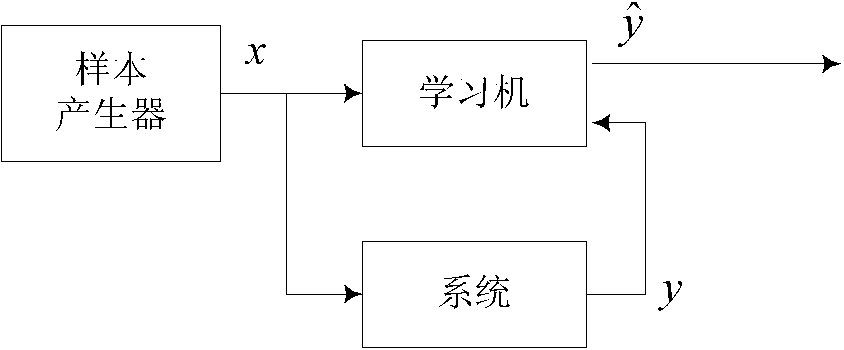
\includegraphics[totalheight=1in]{learn.pdf}
\caption{学习机的结构框图} \label{fig:7-1}
\end{figure}
如图\ref{fig:7-1}所示:
\section{图形并置 \label{chap5:figure2}}
对于比较小的图形我们希望把两个并排放在一起浮动, 且将 \verb/\includegraphics/
命令放到小页环境(miniipage)中可以让用户更好地控制图形的对齐方式.

例如图\ref{fig:7-2}是仅带一个浮动标题的二图并置.
\begin{figure}[ht]
  \centering
  \begin{minipage}[c]{0.5\textwidth}
    \centering
    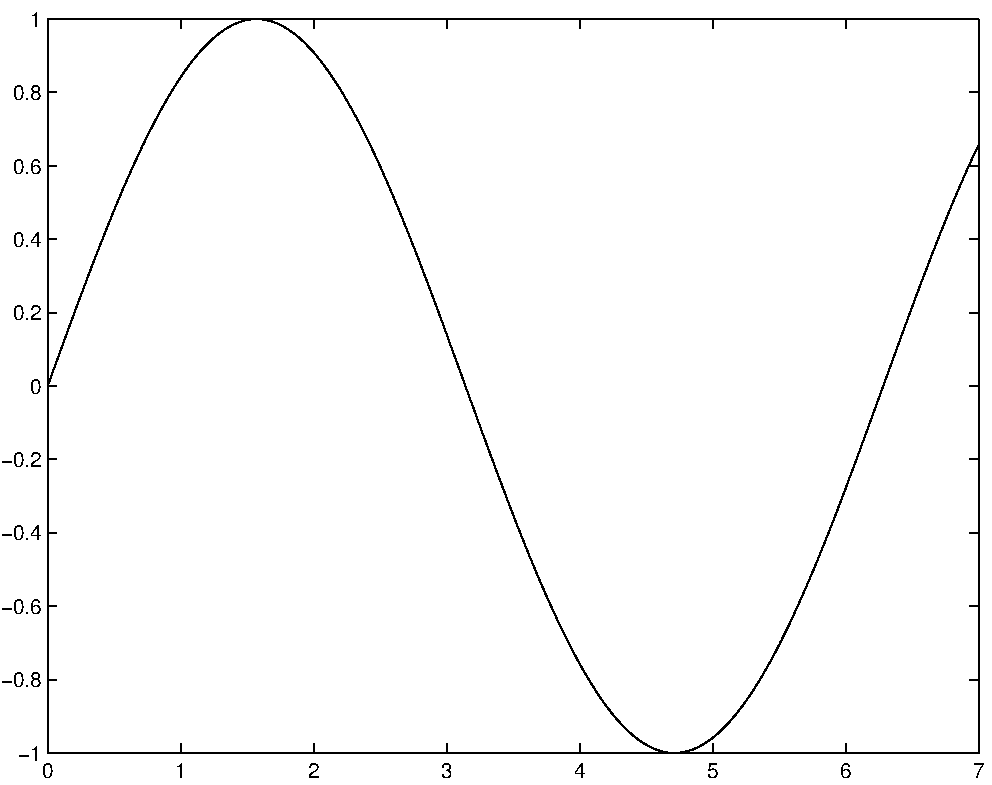
\includegraphics[width=5cm,height=3cm]{sine.pdf}
  \end{minipage}%
  \begin{minipage}[c]{0.5\textwidth}
    \centering
    \includegraphics[width=4cm,height=3cm]{Learn.pdf}
  \end{minipage}
  \caption{采用同个活动标题\label{fig:7-2}}
\end{figure}


下面产生的两图也并列(图\ref{fig:float2-1}和图\ref{fig:float2-2}), 但是有各自的图形标题.
\begin{figure}[ht]
\begin{minipage}[t]{0.45\linewidth}
\centering
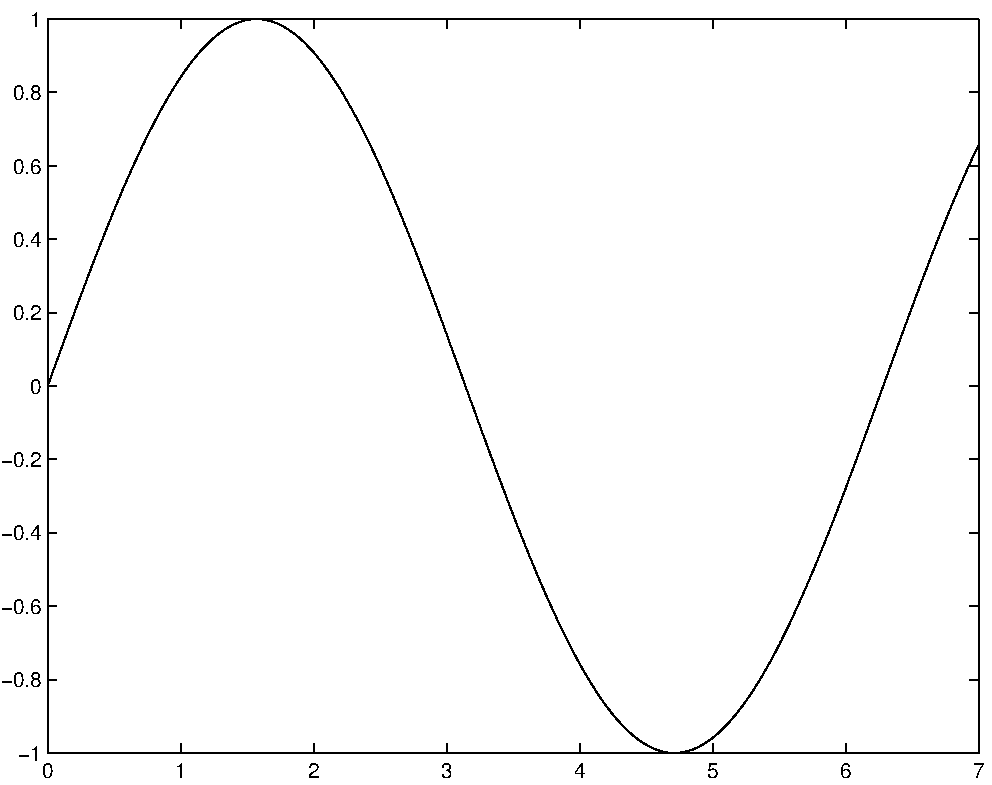
\includegraphics[width=5cm,height=3cm]{sine.pdf}
\caption{这是第一个图\label{fig:float2-1}}
\end{minipage}%
\hfill
\begin{minipage}[t]{0.5\linewidth}
\centering
\includegraphics[width=5cm,height=3cm]{Learn.pdf}
\caption{这是第二个图\label{fig:float2-2}}
\end{minipage}
\end{figure}


下面产生的图\ref{mini:subfigs}有二个子图(图\ref{fig:float3-1}和图\ref{fig:float3-2})组成一组,
而其中的每一幅图又保持其相对独立性.

\begin{figure}[t]
  \centering
  \subfigure[这是第一个图\label{fig:float3-1}]{
    \label{mini:suba} %% label for first subfigure
    \begin{minipage}[b]{0.4\textwidth}
      \centering
      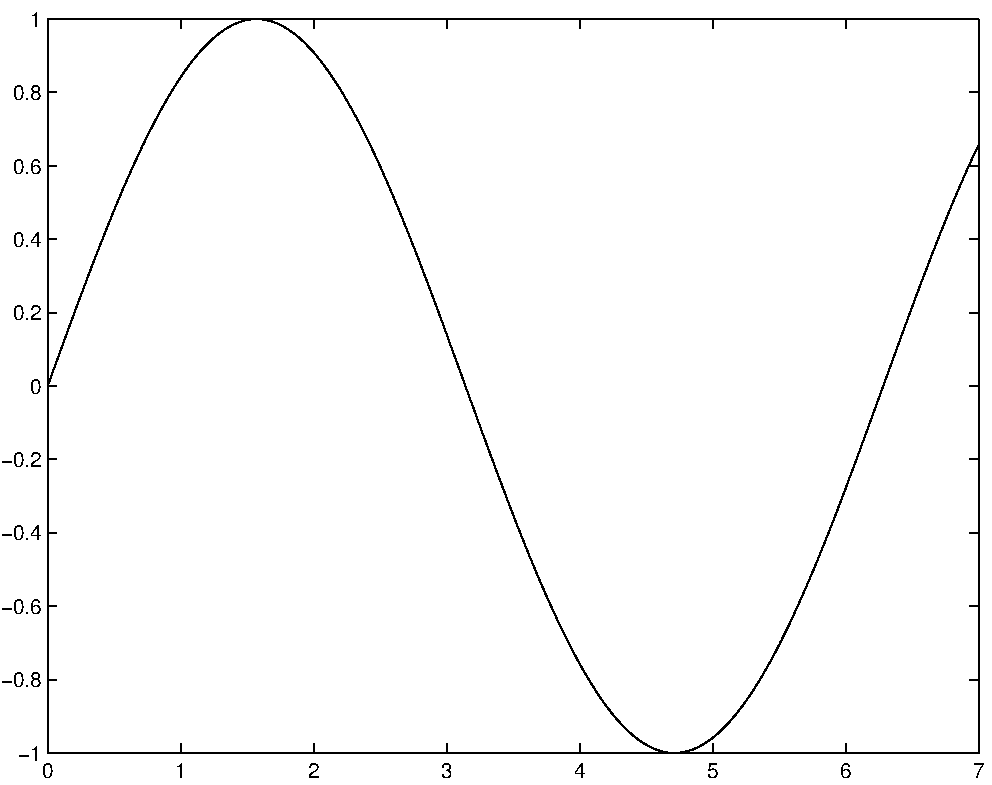
\includegraphics[width=1.5in]{sine.pdf}
    \end{minipage}}%
  \subfigure[这是第一个图\label{fig:float3-2}]{
    \label{mini:subb} %% label for second subfigure
    \begin{minipage}[b]{0.4\textwidth}
      \centering
      \includegraphics[width=1.5in]{Learn.pdf}
    \end{minipage}}
  \caption{二个图形并置}
  \label{mini:subfigs} %% label for entire figure
  \vspace{0.5\textheight}
\end{figure}


% !Mode:: "TeX:UTF-8"
% UTF-8 编辑器
\chapter{数学公式示例}

\setcounter{subsubsection}{0}


\section{单行公式}
\newcommand{\subvec}[3][x]{\ensuremath{#1_{#2},\cdots,#1_{#3}}}


\subsection{类型I: 使用\texttt{equation}单个公式环境}
这种类型使用最为广泛, 可以左对齐(left aligned), 并可自动生成公式编号(和被引用). 其带星号(*)版本则去掉公式编号. Eg.(\ref{eq1})
\begin{equation}\label{eq1}
  x^2+y^2=1
\end{equation}

\subsection{类型II: 使用\texttt{displaymath}环境}
这种类型可以左对齐(left aligned), 但不可自动生成公式编号(和被引用).
\begin{displaymath}
\mu_1\le\mu_2\le\cdots\le\mu_k.
\end{displaymath}

\subsection{类型III: 使用\$\$公式环境}
这种类型只能居中排,可利用命令eqno手工方式加公式编号,但不能被引用.
$$\mu_1\le\mu_2\le\cdots\le\mu_k.\eqno(xx)$$

\subsection{类型IV: 使用 $\backslash[... \backslash]$}
这种类型同上面的类似,可用于临时编绎公式.
\[
\mu_1\le\mu_2\le\cdots\le\mu_k.
\]

\section{多行公式}
\normalsize

\subsection{类型I: 使用\texttt{eqnarray}公式组环境}
这种类型是\texttt{equation}的多行版本, 用于多个公式(方程组)场合. 其带星号(*)版本则去掉公式编号. 若
要去掉其中一个公式编号, 则使用命令\verb=\nonumber=. Eg.(\ref{eq2})和Eg.(\ref{eq3})
\begin{eqnarray}
  x^2+y^2 &=& 1 \label{eq2}\\
  x_2+y_2 &=& 0  \label{eq3}
\end{eqnarray}

\subsection{类型II: 使用\texttt{align}公式组环境}
这种类型与\texttt{eqnarray}类似, 也可自动生成公式编号(和被引用), 差别在于只使用一个\&符号表示上下对齐. 它没有带星号(*)的版本.
Eg.(\ref{eq4})和Eg.(\ref{eq5})
\begin{align}
  x^2+y^2 &= 1 \label{eq4}\\
  x_2+y_2 &= 0  \label{eq5}
\end{align}

\subsection{类型III: 使用\texttt{split}公式组环境}
这种类型实际上是将太长的单行公式分割,  并使用\&符号表示上下对齐. 它不可自动生成公式编号. 但它会与\texttt{ntheorem}冲突.
\begin{verbatim}
\begin{split}
  (x-y)^2&= (x-y)(x-y)\\
         &= x^2 +2 x y +y^2.\\
\end{split}
\end{verbatim}

\subsection{类型IV: 使用displaystyle}
这种类型的公式位置手工安置,可利用命令hss手工方式加贴标签. 公式当然不能深入浮动,因而不能被引用.
这种方式对于非常复杂的多行需要对齐的公式组是一种有效的解决方式.

\vskip\abovedisplayskip \hbox to\hsize{\hskip2cm
  $\displaystyle
y=x
  $\hss (x.1)}
\vskip0.5\baselineskip \hbox to\hsize{\hskip2cm
  $\displaystyle
z=w
  $\hss (x.2)}
\vskip\belowdisplayskip



\subsection{类型V: 使用cases和numcases环境}
这个和array环境一样,可以用\&表示对齐.
不过很重要的一点是, \&之前是数学模式, \&之后是普通的文本模式,数学表达式要写在\$...\$中.
使用numcases环境,需要在导言区 加载宏包cases:
\verb/\usepackage{cases}/或\verb/\usepackage[subnum]{cases}/, 使用前者公式将连续编号,
后者会在同一数字编号后添加a,b等进行编号,本文就是用这种方式编绎的.

下面是四个例子.
\[
f(x)=\begin{cases} 1, & \mbox{If $x\ge 0$}, \\ 0,& \mbox{Otherwise,}\end{cases}
\]

\begin{numcases}{}
a=b & if~$i>j$ \\
c=d & if~$i\leq j$
\end{numcases}

 \begin{numcases}{|x|=}
x, & for $x \geq 0$\\
-x, & for $x < 0$
\end{numcases}

\begin{numcases}{}
u_t-D_j\left(a^{ij}(x,t,u)D_i\varphi(u)\right)\nonumber\\
+b^i(t,u)D_iu+C(x,t,u)=0,&$(x,t)\in B_n\times (0,T)$  \\
u(x,0)=u_{0,n}(x),&  $x\in B_n$   \\
u(x,t)=e^{-\frac{n}{m}},\quad  \mid x \mid =n,& $t>0$
\end{numcases}


\subsection{类型VI: 使用\texttt{align}, \texttt{alignat}, \texttt{aligned}和\texttt{flalign}环境}
它们可用来产生不同的对齐方式,都有星号版本. 现举例说明:
\begin{itemize}
\item[例1:] \texttt{align}: 使用单个\&(带多个编号)
\begin{align}
 y & =d\\
 y & =cx+d\\
 y_{12} & =bx^{2}+ cx+d\nonumber \\
 y(x) & =ax^{3}+ bx^{2}+ cx+d
 \end{align}
\item[例2:] \texttt{align}: 使用3个\&(星号版本)
\begin{align*}
 y & =d & z & =1\\
 y & =cx+d & z & =x +1\\
 y_{12} & =bx^{2}+ cx+d & z & =x^{2}+ x+1 \\
 y(x) & =ax^{3}+ bx^{2}+ cx+d & z & =x^{3}+ x^{2}+ x+1
\end{align*}
\item[例3:] \texttt{alignat}: 产生3个以上对齐(\texttt{align}产生1个或2个对齐)
 \begin{alignat}{3}
 i _{11} & =0.25 & i_{12} & =i_{21} & i_{13} & =i_{23}\nonumber \\
 i _{21} & =\frac{1}{3} i_{11} & i_{22} & =0.5 i_{12}& i_{23} & =i_{31}\\
 i _{31} & =0.33 i_{22}\quad & i_{32} & =0.15 i_{32}\quad & i_{33} & =i_{11}
 \end{alignat}
\item[例4:] \texttt{aligned}: 使用3个\&(仅有一个公式编号)
\begin{equation}
 \begin{aligned}
 2x+3 &= 7 & 2x+3 -3 &= 7-3 \\
 2x &= 4 & \frac{2x}{2} &= \frac42\\
 x &= 2
 \end{aligned}
 \end{equation}
 \item[例5:] \texttt{flalign}: 使用单个\&(居中)
\begin{flalign}\label{eq:centered-1}
 f(x) & = \int \frac{1}{x^2}\ , dx
 \end{flalign}
 \item[例6:] \texttt{flalign}: 使用2个\&(左对齐)
\begin{flalign}\label{eq:centered-2}
 f(x) & = \int \frac{1}{x^2}\ , dx &
 \end{flalign}
 \item[例7:] \texttt{flalign}: 使用3个\&(文本左对齐,公式右对齐)
\begin{flalign*}
 && 12(x -1) +20(y -3) +14(z -2) &= 0\\
 \text{也即} && 6x+10 y+7z &= 50
 \end{flalign*}
\end{itemize}

\subsection{数学公式中的字体}
\newcommand\axy{2\ Greeks,\ \gamma\ and\ \Gamma}
\setlength{\extrarowheight}{-2mm}
\begin{table}[htbp]
\centering
{\small
\caption{数学字体\label{table:mathfont}}
\begin{tabular}{lll}
命令形式   &  意义     &   结果   \\
\toprule
\verb/\mathit{a}/ &  math italic  & $\mathit{\axy}$\\
\verb/\mathnormal{a}/ &  math italic  & $\mathnormal{\axy}$\\
\verb/\mathbf{a}/ &  math bold (upright)    & $\mathbf{\axy}$\\
\midrule
\verb/\mathsf{a}/ &  math san serif  & $\mathsf{\axy}$\\
\verb/\mathrm{a}/ &  math roman  & $\mathrm{\axy}$\\
\verb/\mathtt{a}/ &  math typewriter  & $\mathtt{\axy}$\\
\midrule
\verb/\mathcal{a}/ &  math calligraphic  & $\mathcal{ABC\ R\ XYZ}$\\
\verb/\mathfrak{a}/ &  math Euler Fraktur  & $\mathfrak{123\ abc\ ABC\ R\ XYZ}$\\
\verb/\mathbb{a}/ &  math blackboard bold  & $\mathbb{ABC\ R\ XYZ}$\\
\verb/\mathscr{a}/ &  math blackboard bold  & $\mathscr{ABC\ R\ XYZ}$\\
\midrule
\verb/\boldsymbol{a}/ &  math bold italic    & $\boldsymbol{\axy}$\\
\verb/\boldsymbol{\mathcal{a}}/ &  math calligraphic  & $\boldsymbol{\mathcal{ABC\ R\ XYZ}}$\\
\verb/\bm{a}/ &  bold math & $\bm{\axy}$\\
\bottomrule
\end{tabular}}
\end{table}

\section{方程式编号}
这里提供各种编号的打印方法。

\addtocounter{equation}{1}
\subsection{自动编号的单个的公式}
\begin{equation}
   \subvec [A]{ij}{lk}
\end{equation}
\begin{equation}
   \subvec [A]{ij}{lk}
\end{equation}
\begin{equation}
   \subvec [A]{ij}{lk}
\end{equation}
\subsection{自动编号的公式组:  单一数字编号}
\begin{equation} \label{eq:2}
\begin{split}
y'&= dy / dx \\
 &= f'(x)
 \end{split}
 \end{equation}
\begin{equation} \label{eq:3}
\left\{ \begin{aligned}
         \pi &= 3.141\cdots \\
     \sqrt{2}&=1.414\cdots
        \end{aligned} \right.
\end{equation}
\subsection{自动编号的公式组:  多个数字编号}
\begin{eqnarray}
% \nonumber to remove numbering (before each equation)
  \subvec ij &=& \subvec ij \\
  \subvec ij &=& \subvec ij
\end{eqnarray}

\section{公式的编号与引用}
\subsection{公式引用的基本格式}
公式引用之前必须先在公式环境中添加公式的标记(label):\verb+\label{eq:no}+,其中eq:no表示你给的公式编号,
之后你就可以引用它了.对公式的引用可以采用两种方式:
\begin{enumerate}
\item \verb+\ref{eq:no}+:~这种方式在公式编号的左右不自动添加圆括号,若需要你手工添加,如用\verb+(\ref{eq:3})+产生上面公式的引用(\ref{eq:3}).
\item \verb+\eqref{eq:no}+:~这种方式在公式编号的左右自动添加圆括号,如用\verb+\eqref{eq:3}+同样产
生上面公式的引用\eqref{eq:3}.
\end{enumerate}
\subsection{编号形式的修改}
article文档类使用可选项(leqno)可将公式的位置放在公式的左侧(reqno,缺省)

在文档类article下, 可在导言区通过下面的命令将通篇的公式编号(1), (2), \dots, (100),
随节进行分别编号成(1.1), (1.2), \dots, (5.10).
\begin{verbatim}
   \numberwithin{equation}{section}
\end{verbatim}
若要将公式编号排成(1-1), (1-2), \dots, (5-10)的式样, 可通过自定义命令\verb/\renewcommand/对方程计数器\verb/\theequation/进行修改:
\begin{verbatim}
  \renewcommand\theequation{\thesection-\arabic{equation}}
\end{verbatim}

本节主要讲解子公式编号的建立与引用方法. 
\subsection{子公式的引用}
\subsubsection{使用tag命令修改被引用的公式编号}
\begin{equation}\label{E:first}
A^{[2]} \diamond B^{[2]} \cong (A \diamond B)^{[2]}
\end{equation}
\begin{equation}\tag{\ref{E:first}$'$}\label{E:new}
A^{\langle 2 \rangle} \diamond B^{\langle 2\rangle}
\equiv (A \diamond B)^{\langle 2 \rangle}
\end{equation}
使用tag命令后的公式引用方法为: \verb/(\ref{E:first}$'$)/ 或 \verb/\eqref{E:new}/, 得到(\ref{E:first}$'$), \eqref{E:new}.
这时原有方程计数器的值并不增加.

\subsubsection{使用subequations数学环境(需要amsmath宏包支持)}
\begin{subequations}\label{E-T}
\begin{equation}\label{E-O}
A^{[2]} \diamond B^{[2]} \cong (A \diamond B)^{[2]}
\end{equation}
\begin{equation}\label{E-M}
A^{\langle 2 \rangle} \diamond B^{\langle 2\rangle}
\equiv (A \diamond B)^{\langle 2\rangle}
\end{equation}
\end{subequations}
引用: 由\verb/\eqref{E-T}/, \verb/\eqref{E-O}/, \verb/\eqref{E-M}/主公式与子公式的浮动引用:
\eqref{E-T}, \eqref{E-O}, \eqref{E-M}.

\subsubsection{使用align或gather环境(需要amsmath宏包支持)}
更为方便的办法是用align或gather环境代替上面subequations环境中的多个equation环境.
\begin{subequations}\label{EE}
\begin{align}
y&=cx+d \label{E1}\\
y&=bx^2+cx+d \label{E2}\\
y&=ax^3+bx^2+cx+d \label{E3}
\end{align}
\end{subequations}
公式引用:\eqref{EE},\eqref{E1}, \eqref{E2},\eqref{E3}.

\begin{subequations}\label{E:gp}
\begin{gather}
y=cx+d \label{gp1}\\
y=bx^2+cx+d \label{gp2}\\
yax^3+bx^2+cx+d \label{gp3}
\end{gather}
\end{subequations}
%愈来愈不具体通过性.

\subsubsection{使用subeqnarray数学环境(需要subeqnarray宏包支持)}
subeqnarray宏包提供了subeqnarray和subeqnarray*数学环境.
\begin{subeqnarray}
\label{eqw}
x & = & a \times b \slabel{eq-a}\\
& = & z + t \slabel{eq-b}\\
& = & z + t \slabel{eq-c}
\end{subeqnarray}
方程的整体引用与单独引用可分别通过\verb/\eqref{eqw}/, \verb/\eqref{eq-a}/,  \verb/\eqref{eq-b}/,  \verb/\eqref{eq-c}/实现:
~\eqref{eqw}, \eqref{eq-a}, ~\eqref{eq-b},~\eqref{eq-c}.

%subeqn 也可以!!

\subsubsection{使用subnumcases设定多行分支公式的编号(需要cases宏包支持)}
\begin{subnumcases}{\label{WW}|x|=}
x, & for  $x\geq 0$ \label{W-a} \\
-x, & for  $x<0$ \label{W-b}
\end{subnumcases}
比较: 使用subnumcases数学环境可产生三个可浮动引用的公式编号, 一个主编号, 二个子编号, 而普通的cases环境在equation环境中仅产生一个
可浮动引用的公式编号, cases宏包中的numcases数学环境可产生二个连续的公式编号.

上面公式引用: \verb/\eqref{WW}, \eqref{W-a}, \eqref{W-b}/后的结果为
\eqref{WW}, \eqref{W-a}, \eqref{W-b}.



% !Mode:: "TeX:UTF-8"
% UTF-8 编辑器
\chapter{定理型声明示例}
\section{自动编号的声明}
\begin{definition} %
\aaa
\end{definition}%
\begin{proposition} %
\aaa
\end{proposition}%
\begin{theorem}%
 \aaa
\end{theorem}%
\begin{example}%
\aaa
\end{example}
\begin{lemma}%
\aaa
\end{lemma}
\begin{axiom}%
\aaa
\end{axiom}
\begin{corollary}%
\aaa
\end{corollary}
\begin{exercise}%
\aaa
\end{exercise}
\begin{proof}%
\aaa
\end{proof}

%\include{body/fonts}
%------公式,参考文献的标签显示在页边,在论文修改时可以使用------
%\include{body/labelname}

% !Mode:: "TeX:UTF-8"
% UTF-8 编辑器
\chapter{关于参考文献}

其中~chinesebst~是清泉自己所生成的参考文献风格,比较符合中国人的习惯。
\section{引用格式的修改1}

第一行在引用处数字两边加方框

第二行去除参考文献里数字两边的方框

\begin{verbatim}
\makeatletter
\def\@cite#1{\mbox{$\m@th^{\hbox{\@ove@rcfont[#1]}}$}}
\renewcommand\@biblabel[1]{#1}
\makeatother
\end{verbatim}
\section{引用格式的修改2}
\subsection*{增加~$\backslash$ucite~命令使显示的引用为上标形式}
使用下面的一种定义方法:
\begin{verbatim}
\newcommand{\ucite}[1]{$^{\mbox{\scriptsize \cite{#1}}}$}
\end{verbatim}
\begin{verbatim}
\newcommand{\ucite}[1]{\textsuperscript{\textsuperscript{\cite{#1}}}}
\end{verbatim}
\section{引用示例}
一般引用 \verb"\cite{Wang2}"
产生如:\cite{Wang2}. 包含正文中没有引用的文献可以使用\verb/\nocite{Xiedy1997}/产生~\nocite{Xiedy1997}.

上标引用 \verb"\ucite{Wang1}",产生如:\ucite{Wang1}

多个连续引用

\verb"\cite{CTug,Sangdy,Wang2,net1,net2,net3}",

产生如:\cite{CTug,Sangdy,Wang2,net1,net2,net3}.


多个上标连续引用

\verb"\ucite{CTug,Sangdy,Wang2,net1,net2,net3}",

产生如:\ucite{CTug,Sangdy,Wang2,net1,net2,net3}.


%建立索引的例子,需要在运行LaTeX(PDFLaTeX)后,运行 MakeIndex
%% !Mode:: "TeX:UTF-8"
% UTF-8 编辑器
\chapter{索引示例}

这是一个主条目1。\index{主条目1}

这是一个主条目2。\index{主条目2}

这是一个子条目1。\index{主条目2!子条目1}

这是一个子条目2。\index{主条目2!子条目2}

这是一个子条目3。\index{主条目2!子条目3}

这是一个子条目4。\index{主条目2!子条目4}

这是一个子子条目1。\index{主条目2!子条目4!子子条目1}

这是一个子子条目2。\index{主条目2!子条目4!子子条目2}

这是一个子子条目3。\index{主条目2!子条目4!子子条目3}

这是一个子子条目4。\index{主条目2!子条目4!子子条目4}

这是一个主条目3。\index{主条目3}

这是一个主条目4。\index{主条目4}



%结论
% !Mode:: "TeX:UTF-8"
% UTF-8 编辑器

\defaultfont

\chapter*{结~~~~论}
\markboth{结~~~~论}{结~~~~论}
\addcontentsline{toc}{chapter}{\bf 结论}

本论文提供了一个完整的华东师范大学博士(硕士)论文模板. 这套模板符合
学校的有关要求, 方便易用. 这一工作对广大研究生更好地撰写学位论文无疑
带来很大的便利, 在其它场合同样会发挥重要的作用. 


%附录
%----------- 定义附录中的标题、图形、表格、公式的编号格式 -------------------%
\begin{appendix}
    \renewcommand{\chaptername}{附录 \Alph{chapter}}
    \renewcommand{\thesection}{\Alph{chapter}.\arabic{section}}
    \renewcommand{\thesubsection}{\Alph{chapter}.\arabic{section}.\arabic{subsection}}
    \renewcommand{\thesubsubsection}{\arabic{subsubsection}.}
    \renewcommand{\thetable}{\Alph{chapter}-\arabic{table}}
    \renewcommand{\theequation}{\Alph{chapter}-\arabic{equation}}
    \renewcommand{\thefigure}{\Alph{chapter}-\arabic{figure}}
%   \input{appendix/A01}
%   \input{appendix/A03}
   % !Mode:: "TeX:UTF-8"
% UTF-8 编辑器
%%%%%%%%%%%%%%%%%%%%%%%%%%%%%%%%%%%%%%%%%%%%%%%%%%%%%%%%%%%%%%%%%%%%%%%%%

%   LaTeX File for Doctor (Master) Thesis of Tsinghua University
%   LaTeX + CJK     上海师范大学博士(硕士)论文模板
%   Based on Wang Tianshu's Template for XJTU
%   Version: 1.00
%   Last Update: 2003-09-12
%%%%%%%%%%%%%%%%%%%%%%%%%%%%%%%%%%%%%%%%%%%%%%%%%%%%%%%%%%%%%%%%%%%%%%%%%
%
%   LaTeX File for Doctor (Master) Thesis of Tsinghua University
%   LaTeX + CJK     华东师范大学博士(硕士)论文模板
%   Based on Wang Tianshu's Template for XJTU
%   Version: 1.65
%   Last Update: 2005-05-10
%
%%%%%%%%%%%%%%%%%%%%%%%%%%%%%%%%%%%%%%%%%%%%%%%%%%%%%%%%%%%%%%%%%%%%%%%%%%%%%%%%%%%%
%   Copyright 2002-2005  by  Yincai Tang (tangyc8866)       (tangyc8866@hotmail.com)
%%%%%%%%%%%%%%%%%%%%%%%%%%%%%%%%%%%%%%%%%%%%%%%%%%%%%%%%%%%%%%%%%%%%%%%%%%%%%%%%%%%%

\defaultfont

\chapter{相关数学公式和证明}
加油! 终于到最后一个部分了!
\section{附录中的图形、表格、公式}
在附录出现之前添加下面的命令
\begin{verbatim}
%--------------定义附录中的图、表、公式的编号格式 --------------%
\renewcommand{\thetable}{\Alph{chapter}-\arabic{table}}
\renewcommand{\theequation}{\Alph{chapter}-\arabic{equation}}
\renewcommand{\thefigure}{\Alph{chapter}-\arabic{figure}}
\renewcommand{\chaptername}{附录\Alph{chapter}}
\renewcommand{\thesection}{\Alph{chapter}.\arabic{section}}
%--------------------%%%%%%%%%%%%%%%%-----------------------%
\end{verbatim}
就可实现公式表格和图形的重新编号及引用.

例如附录中的公式(\ref{equ:Call})和(\ref{equ:Put})分别为:
\begin{equation}\label{equ:Call}
  c=S_0N(d_1)-X e^{-r T}N(d_2)
\end{equation}
和
\begin{equation}\label{equ:Put}
  p=X e^{-r T}N(-d_2)-S_0N(-d_1),
\end{equation}


\end{appendix}


\backmatter %结束章节自动编号

%其中chinesebst是我自己生成的参考文献风格,比较符合中国人的习惯
%参考文献
%\bibliographystyle{cnbst}
%\phantomsection
%\bibliography{reference/reference,reference/chinese,reference/english}
%\bibliography{reference/ref}

\addcontentsline{toc}{chapter}{参考文献}
% !Mode:: "TeX:UTF-8"
% UTF-8 编辑器
\begin{thebibliography}{99}
%\setlength{\parskip}{0pt}  %段落之间的竖直距离
\addtolength{\itemsep}{-0.8 em} % 缩小参考文献间的垂直间距
  \bibitem{Art}  作者, ~~文章题目, ~~{\it 期刊名称}, {\bf 卷号(期数)}(年份), 起始页码.
  \bibitem{Book}  作者, ~~{\it 书名}, 出版社, 年份.
  \bibitem{Conference}  作者, ~~文章题目, {\it 论文集名}, 编者, 出版社, 年份, 起始页码.
  \bibitem{Xiedy1997}  薛定宇, ~~{\it \LaTeX 科学文件处理软件入门(修订版)}, 1997.
  \bibitem{Dengjs} 邓建松, 彭冉冉, 陈长松, ~~{\it \LaTeX2e科技排版指南}, 2001.
  \bibitem{Sangdy} 桑大勇, 王瑛, ~~{\it  科技文献排版系统:\LaTeX 入门与提高}, 2001.
  \bibitem{Chenzj} 陈志杰, 赵书钦, 万福永, ~~{\it  \LaTeX 入门与提高}, 高等教育出版社, 2002.
  \bibitem{Wang1} K. Reckdahl~原著,王磊 译, ~~{\it  Using Import graphics in \LaTeX2e}, 2000.
  \bibitem{Wang2}王 磊, ~~{\it LATEX2e 插图指南}.
  \bibitem{texguru} \TeX Guru 译, ~~{\it \LaTeX2e 用户手册}, 1999.8.15
  \bibitem{daly} Patrick W. Daly, Graphics and Colour with \LaTeX, 1998.4
  \bibitem{CTug} Tobias Oetiker~原著, ChinaTeX用户小组译, ~~{\it  一份不太简短的LATEX2e介绍}, 2002.
  \bibitem{TexFriend03}Mytex, ~~{\it  TexFriend/Graphics插件}, 2003. http://www.ctex.org/forums/
  \bibitem{Lisj}李树钧, ~~{\it  fixbbl:BibTEX的中文本地化解决方案}, 2003. http://www.hooklee.com
  \bibitem{Kabal}Peter Kabal, \TeX draw: PostScript Drawings from \TeX, Edition 2.1, 1999
  \bibitem{net1}http://tex.loria.fr/english/prod-graph.html
  \bibitem{net2}http://tex.loria.fr/graph-pack/grf/grf.htm
  \bibitem{net3} http://www.ctex.org/forums/index.php?showtopic=9532
\end{thebibliography}


%索引
\newpage
\printindex %该命令可以放到想要出现索引列表的地方
\addcontentsline{toc}{chapter}{索\ 引}

%致谢
% !Mode:: "TeX:UTF-8"
% UTF-8 编辑器

%%%%%%%%%%%%%%%%%%%%%%%%%%%%%%%%%%%%%%%%%%%%%%%%%%%%%%%%%%%%%%%%%%%%%%%%%%%%%%%%%%%%
%   Copyright 2002-2005  by  Yincai Tang (tangyc8866)       (tangyc8866@hotmail.com)
%%%%%%%%%%%%%%%%%%%%%%%%%%%%%%%%%%%%%%%%%%%%%%%%%%%%%%%%%%%%%%%%%%%%%%%%%%%%%%%%%%%%

\acknowledge{
从200x年9月至今的三年学习期间得到了数理信息学院许多老师、同学和朋友的帮助, 在此一并表示感谢.

\hspace{2\ccwd}在论文的选题到完成的各个阶段, 自始自终得到了导师 xxx
的细心指导和帮助, 并提供了许多宝贵的资料和建议, 其......和严谨的治学精神是我整整三年学习期间最为珍贵的养份,
在此我想由忠地说一声:谢谢 xxx 老师, 谢谢你给我的无私的帮助!

\hspace{2\ccwd}最后, 也是最为重要的, 我的 xxx 多年来一直支持我的学习和研究, 在论文的完成过程中付出了大量的时间和心血. 
感激之情, 难以言表, 我将永身不忘.}


%发表的文章列表
% !Mode:: "TeX:UTF-8"
% UTF-8 编辑器

%%%%%%%%%%%%%%%%%%%%%%%%%%%%%%%%%%%%%%%%%%%%%%%%%%%%%%%%%%%%%%%%%%%%%%%%%%%%%%%%%%%%
%   Copyright 2002-2005  by  Yincai Tang (tangyc8866)       (tangyc8866@hotmail.com)
%%%%%%%%%%%%%%%%%%%%%%%%%%%%%%%%%%%%%%%%%%%%%%%%%%%%%%%%%%%%%%%%%%%%%%%%%%%%%%%%%%%%


\defaultfont

\chapter*{在学期间的研究成果及发表的论文}
\markboth{在学期间的研究成果及发表的论文}{在学期间的研究成果及发表的论文}
\addcontentsline{toc}{chapter}{\bf 在学期间的研究成果及发表的论文}

\section*{在国际和国内学术刊物上发表的论文}

\renewcommand{\labelenumi}{[\arabic{enumi}]}

\begin{enumerate}

\item L. Wang, S. Kang, H. Shum, G. Xu, Error Analysis of Pure
Rotation-based Self-Calibration, {\em{IEEE Transactions on Pattern
Analysis and Machine Intelligence (PAMI)}}, in press

\item xxxx, xxx,xxx. 一种基于全景图的三维房间导航方法.
软件学报, 2002, 13(Suppl.): 31-35

\end{enumerate}

\section*{在国际和国内学术会议上发表的论文}

\begin{enumerate}

\item L. Wang, S. Kang, H. Shum, G. Xu, Error Analysis of Pure
Rotation-based Self-Calibration, {\em{in Proceedings of the Eighth
IEEE International Conference on Computer Vision(ICCV'01)}}, I:
464-471, Vancouver, BC, Canada, July, 2001

\item L. Wang, X. Liu, L. Xia, G. Xu, A. Bruckstein, Image
Orientation Detection with Integrated Human Perception Cues,
{\em{in Proceedings of IEEE International Conference on Image
Processing (ICIP'03)}}, in press

\end{enumerate}


\clearpage
\end{document}

%%%%%%%%%%%%%%%%%% End of the file  %%%%%%%%%%%%%%%%%%%%%%%%
